\part{Software Architecture}

Before writing the code for the demos, we started by coming up with an
overall software architecture.  The purpose of this planning was to
write each node so that as other nodes are added to our software
package we do not have to spend time rewriting old code.

This section will describe the decisions we made and what we have
planned.

\section{Node Architecture}
\todo[inline]{Show and describe the data from the software
  architecture diagram.  The visio file David made will probably need
  to be updated. We'll also want to show the end goal and what we
  currently have implemented}

The main document we are basing our software architecture off of is
the following:

\begin{figure}[h]
  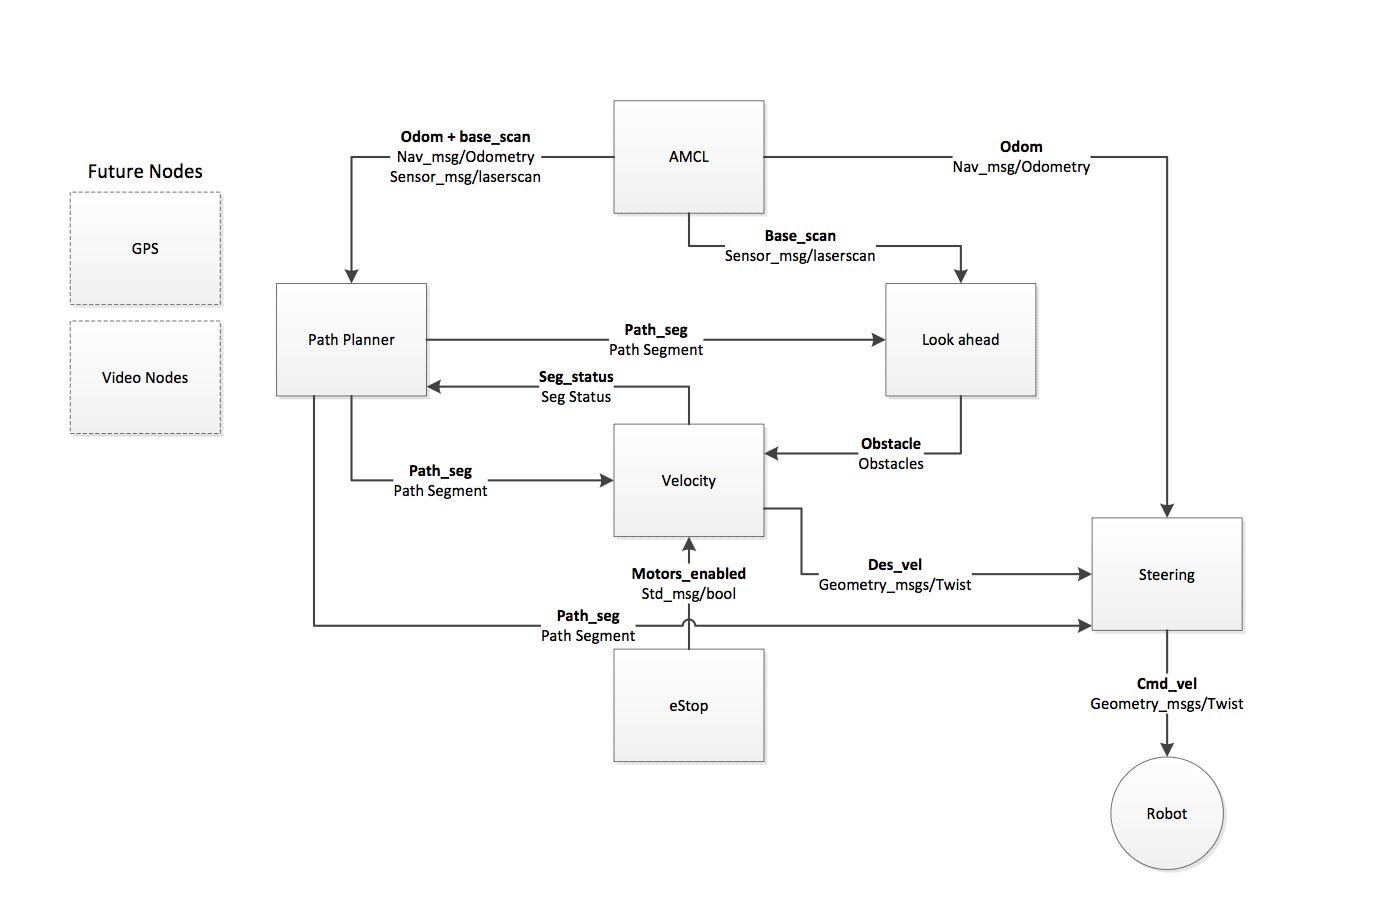
\includegraphics[width=8.0in]{software_architecture_diagram}
  \caption{Planned Software Architecture}
\end{figure}
\missingfigure{Add the image of the communications diagram}

This figure clearly shows the different nodes we have planned, the
communication message types being passed between them, and areas of
possible future expansion.

The specifications for the nodes in the diagram and the messages being
used will be found in the rest of this section.

\section{Packaging and Stacks}
\todo[inline]{Information about how we split the nodes into different
  packages}
\todo[inline,color=green]{Mark should take care of this}

\section{Node Specifications}
\todo[inline]{Formal spec for each node that is planned}

To help guide us while writing our nodes we wrote a small
specification for each class seen in the software architecture diagram.

\subsection{Velocity Profiler}
This node is at the heart of the robot.  Nothing gets done without the
velocity profiler node running.  This node is responsible for taking
in path segments and calculating spatial trajectories.  The desired
velocities at each point along the path must obey all of the path
constraints specified by the path segment.  Path segments must be

\subsubsection{Requirements}
\begin{enumerate}
  \item Velocity Profiler must accept PathSegment messages from
    Path Planner
    \item Velocity Profiler must calculate spatial trajectories from
      the accepted PathSegment messages
      \begin{enumerate}
        \item Velocity Profiler must obey all of the path constraints
          specified in every accepted PathSegment message
         \end {enumerate}
\item Velocity Profiler must respond to Obstacle messages from Look
  Ahead
  \begin{enumerate}
    \item Velocity Profiler must stop and wait at an obstacle for a
      specified amount of time
      \item Velocity Profiler must alert Path Planner if an obstacle
        has not moved after a specified time
      \end{enumerate}
      \item Velocity Profiler must publish a desired velocity based on
        the robots current position
      \item Velocity Profiler must stop when the E-Stop is enabled
        \item Velocity Profiler must resume a plan after the E-Stop is
  disabled
  \end{enumerate}
      
\subsection{Look Ahead}

\subsection{Steering}

\subsection{Path Planning}

\subsection{Video}

\subsection{Sensors}
\todo[inline]{Talk about the other sensors, e.g. GPS. This will
  probably be rolled into the other nodes as the cRIO should take care
  of most of this}

\section{Custom Message Specifications}
\todo[inline]{Formal spec for each message that is planned. This will
  essentially be the .msg file}

\subsection{segStatus}

\subsection{obstacles}

\section{Topics}
\todo[inline]{Short description of what each topic is publishing and why}

\subsection{des\_vel}

\subsection{cmd\_vel}

\subsection{base\_laser1\_scan and base\_scan}

\subsection{seg\_status}

\subsection{path\_seg}